\documentclass{beamer}
\usepackage[T1]{fontenc}
\usepackage[utf8]{inputenc}

\usetheme{Madrid}
\usecolortheme{default}
\usepackage{amsmath,amssymb,amsfonts,amsthm}
\usepackage{txfonts}
\usepackage{tkz-euclide}
\usepackage{listings}
\usepackage{adjustbox}
\usepackage{array}
\usepackage{tabularx}
\usepackage{gvv}
\usepackage{lmodern}
\usepackage{gensymb}
\usepackage{circuitikz}
\usepackage{tikz}
\usepackage{graphicx}
\usepackage{capt-of}

\setbeamertemplate{page number in head/foot}[totalframenumber]

\usepackage{tcolorbox}
\tcbuselibrary{minted,breakable,xparse,skins}

\definecolor{bg}{gray}{0.95}
\DeclareTCBListing{mintedbox}{O{}m!O{}}{%
  breakable=true,
  listing engine=minted,
  listing only,
  minted language=#2,
  minted style=default,
  minted options={%
    linenos,
    gobble=0,
    breaklines=true,
    breakafter=,,
    fontsize=\small,
    numbersep=8pt,
    #1},
  boxsep=0pt,
  left skip=0pt,
  right skip=0pt,
  left=25pt,
  right=0pt,
  top=3pt,
  bottom=3pt,
  arc=5pt,
  leftrule=0pt,
  rightrule=0pt,
  bottomrule=2pt,
  toprule=2pt,
  colback=bg,
  colframe=orange!70,
  enhanced,
  overlay={%
    \begin{tcbclipinterior}
    \fill[orange!20!white] (frame.south west) rectangle ([xshift=20pt]frame.north west);
    \end{tcbclipinterior}},
  #3,
}
\lstset{
    language=C,
    basicstyle=\ttfamily\small,
    keywordstyle=\color{blue},
    stringstyle=\color{orange},
    commentstyle=\color{green!60!black},
    numbers=left,
    numberstyle=\tiny\color{gray},
    breaklines=true,
    showstringspaces=false,
}

\title{4.5.12}
\subtitle{Equation of plane}
\author{EE25BTECH11010 - Arsh Dhoke}
\date{}
\begin{document}


\begin{frame}
  \titlepage
\end{frame}


\begin{frame}{Question}
Find the equation of the plane passing through 
$(a,b,c)$ and parallel to the plane $\vec{r}\cdot(\vec{i}+\vec{j}+\vec{k})=2$
\end{frame}
\begin{frame}{Input parameters}
\begin{tabular}{|c|c|}
\hline
\textbf{Name} & \textbf{Value} \\ \hline
$\vec{A}$ & $\myvec{2 & 1 \\0 & 3}$ \\ \hline
\end{tabular}

\end{frame}
\begin{frame}{Solution}
Given plane:
\begin{align}
\vec{n}^T \vec{x} = 2
\end{align}

Required plane (parallel to given plane):
\begin{align}
\vec{n}^T \vec{x}=d
\end{align}
\end{frame}

\begin{frame}{Finding $d$}
Substitute given point in required plane:
\begin{align}
\myvec{1&1&1}\cdot\myvec{a\\b\\c}=d
\end{align}

Thus,
\begin{align}
d=a+b+c
\end{align}
\end{frame}

\begin{frame}{Final answer}
\boxed{\vec{n}^T \vec{x}=a+b+c} \\

This can also be written in the form:
\boxed{\vec{r}\cdot\myvec{1\\1\\1}=a+b+c}
    
\end{frame}

\begin{frame}{Plot}
\begin{figure}
\centering
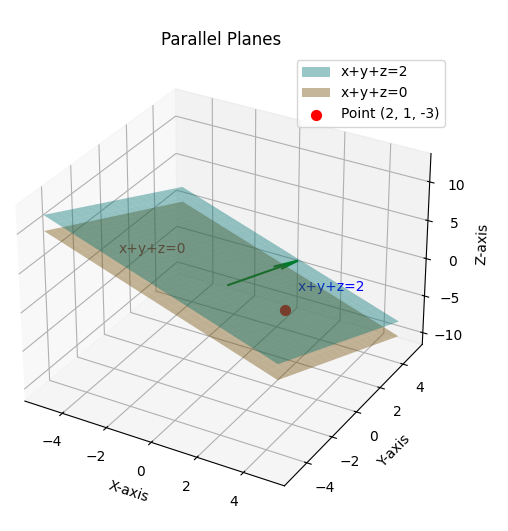
\includegraphics[height=0.6\textheight, keepaspectratio]{figs/q7.png}
\captionof{figure}{Graph}
\end{figure}
\end{frame}

\begin{frame}[fragile]
    \frametitle{C Code}
\begin{lstlisting}
#include <stdio.h>

double plane_equation(double a, double b, double c) {
    return a + b + c;
}

\end{lstlisting}
\end{frame}

\begin{frame}[fragile]
    \frametitle{Python Code}
\begin{lstlisting}
import numpy as np
import matplotlib.pyplot as plt

def plane_equation(point):
    """Returns d for the plane x + y + z = d through point (a, b, c)."""
    a, b, c = point
    return a + b + c

def plot_planes(point):
    # Normal vector
    n = np.array([1, 1, 1])
    
    # Given plane: x + y + z = 2
    d1 = 2
    
    # Required plane: x + y + z = a+b+c
    d2 = plane_equation(point)
    \end{lstlisting}
\end{frame}

\begin{frame}[fragile]
    \frametitle{Python Code}
\begin{lstlisting}
    # Meshgrid for plotting
    x = np.linspace(-5, 5, 20)
    y = np.linspace(-5, 5, 20)
    X, Y = np.meshgrid(x, y)
    
    # z for each plane
    Z1 = (d1 - X - Y) / n[2]
    Z2 = (d2 - X - Y) / n[2]
    
    # Plot
    fig = plt.figure(figsize=(8, 6))
    ax = fig.add_subplot(111, projection='3d')
    
    # Given plane
    ax.plot_surface(X, Y, Z1, alpha=0.4, color='cyan', label="x+y+z=2")
    ax.text(2, 2, (d1 - 2 - 2), "x+y+z=2", color='blue', fontsize=10)
 \end{lstlisting}
\end{frame}
    
    \begin{frame}[fragile]
    \frametitle{Python Code}
\begin{lstlisting}
    # Required plane
    ax.plot_surface(X, Y, Z2, alpha=0.4, color='orange', label=f"x+y+z={d2}")
    ax.text(-3, -3, (d2 - (-3) - (-3)), f"x+y+z={d2}", color='brown', fontsize=10)
    
    # Mark the given point with legend
    ax.scatter(point[0], point[1], point[2], color='red', s=50, label=f"Point {point}")
    
    # Normal vector arrow
    origin = np.array([0, 0, 0])
    ax.quiver(*origin, *n, length=2, color="green")
    \end{lstlisting}
\end{frame}

\begin{frame}[fragile]
    \frametitle{Python Code}
\begin{lstlisting}
    # Axes labels
    ax.set_xlabel("X-axis")
    ax.set_ylabel("Y-axis")
    ax.set_zlabel("Z-axis")
    ax.set_title("Parallel Planes")
    
    # Show legend
    ax.legend()
    plt.savefig("/home/arsh-dhoke/ee1030-2025/ee25btech11010/matgeo/4.5.12/figs/q7.png")
    plt.show()

# Example usage
point = (2, 1, -3)  
plot_planes(point)

\end{lstlisting}
\end{frame}

\begin{frame}[fragile]
    \frametitle{Python+ C Code}
\begin{lstlisting}
import ctypes
import numpy as np
import matplotlib.pyplot as plt

# Load the shared library
lib = ctypes.CDLL('./code.so')

# Tell Python about the argument and return types
lib.plane_equation.argtypes = (ctypes.c_double, ctypes.c_double, ctypes.c_double)
lib.plane_equation.restype = ctypes.c_double

# Example point (a,b,c) that lies on the plane
a, b, c = 2.0, 1.0,-3.0

# Use C function to calculate d = a+b+c
d = lib.plane_equation(a, b, c)
print(f"Plane equation: x + y + z = {d}")
\end{lstlisting}
\end{frame}

\begin{frame}[fragile]
    \frametitle{Python+ C Code}
\begin{lstlisting}
# Define a meshgrid for x and y
x_vals = np.linspace(-5, 5, 50)
y_vals = np.linspace(-5, 5, 50)
X, Y = np.meshgrid(x_vals, y_vals)

# Solve for Z using x + y + z = d
Z = d - X - Y

# Plot the plane
fig = plt.figure(figsize=(8,6))
ax = fig.add_subplot(111, projection='3d')
ax.plot_surface(X, Y, Z, alpha=0.7, color="lightblue", edgecolor='k')

# Plot the example point
ax.scatter(a, b, c, color='red', s=50, label=f'Point ({a},{b},{c})')
\end{lstlisting}
\end{frame}

\begin{frame}[fragile]
    \frametitle{Python+ C Code}
\begin{lstlisting}
# Label axes
ax.set_xlabel("X")
ax.set_ylabel("Y")
ax.set_zlabel("Z")
ax.set_title(f"Plane: x + y + z = {d}")

plt.legend()
plt.savefig("/home/arsh-dhoke/ee1030-2025/ee25btech11010/matgeo/4.5.12/figs/q7.png")
plt.show()

\end{lstlisting}
\end{frame}
\end{document}